\begin{flushright} {\tiny {\color{gray} \tt mms\_elsw.tex}} \end{flushright}
%~~~~~~~~~~~~~~~~~~~~~~~~~~~~~~~~~~~~~~~~~~~~~~~~~~~~~~~~~~~~~~~~~~~~~~~~~~~~~~~~~~~~~~~~~~~~~~~~~~

This comes from Elman \etal \cite{elsw}(section 3.1.4)\footnote{actually, not?}. 
The velocity is prescribed to be
\[
{\vec v}=(2y(1-x^2) ; -2x(1-y^2) )
\]
on the domain $\Omega=[-1:1]\times[-1:1]$. The strainrate tensor is given by:
\[
\dot{\bm \varepsilon}=
\left(
\begin{array}{cc}
-4xy & -x^2+y^2  \\
-x^2+y^2 & 4xy   
\end{array}
\right)
\]
The Stokes equation is then:
\begin{eqnarray}
-\frac{\partial p}{\partial x} + 2\eta ( -4y + 2y ) &=& \rho g_x \\
-\frac{\partial p}{\partial y} + 2\eta ( -2x + 4x ) &=& \rho g_y
\end{eqnarray}
where we assume the viscosity $\eta=1$ to be constant in space.
Assuming $g_x=0$, the first equation is
\[
\frac{\partial p}{\partial x} = - 4 y
\]
i.e.
\[
p(x,y)= -4  y x +f(y)
\]
Inserting this in the second equation:
\[
4  x - f'(y) + 4 x  = \rho g_y
\]
or,
\[
-f'(y) + 8  x  = \rho g_y
\]
Assuming $g_y=-1$, we get $\rho=-8x$ and then $f'(y)=0$ so $f(y)=C$ where $C$
is a constant.
Finally the pressure is given by:
\[
p(x,y)=-4  y x + C
\]
We add the following requirement: $\int_\Omega p(x,y) d\Omega =0$ so that $C=0$.

\begin{center}
\includegraphics[width=6cm]{images/benchmark_ldc_anal/velo}
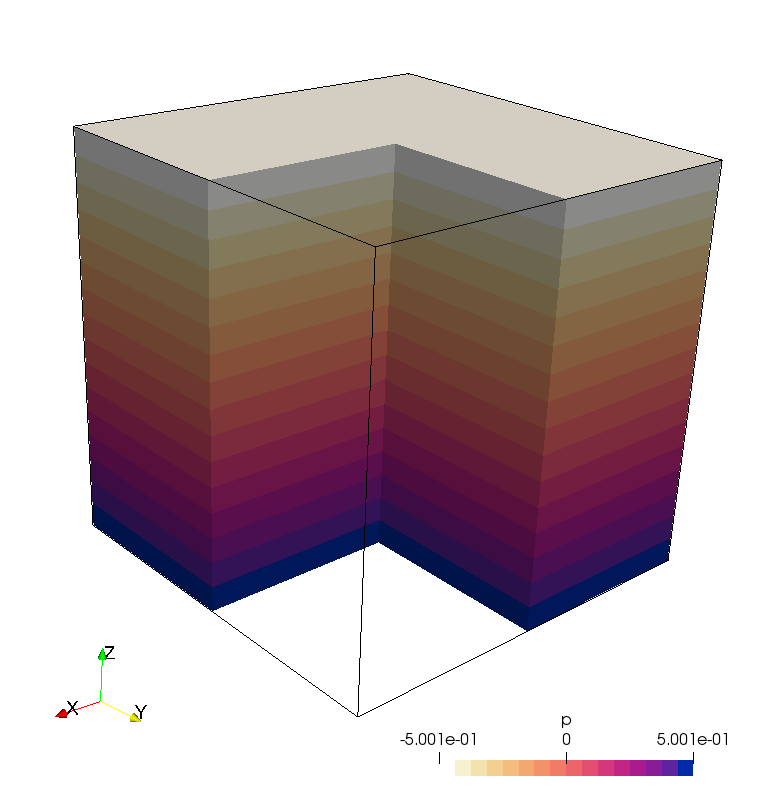
\includegraphics[width=6cm]{images/benchmark_ldc_anal/press}
\end{center}

\begin{eqnarray}
\upnu_{rms}^2 
&=& \frac{1}{\Omega} \int_\Omega (u^2+v^2) d\Omega \nonumber\\
&=& \frac{1}{4} \int_{-1}^{+1}\int_{-1}^{+1} (u^2+v^2) dxdy \nonumber\\
&=& \frac{1}{4} \int_{-1}^{+1}\int_{-1}^{+1} [ 4y^2(1-x^2)^2 + 4x^2(1-y^2)^2   ] dxdy \nonumber\\
&=& \int_{-1}^{+1}\int_{-1}^{+1} [ y^2(1-x^2)^2 + x^2(1-y^2)^2   ] dxdy \nonumber\\
&=& \int_{-1}^{+1}\int_{-1}^{+1} [ y^2(1-2x+x^2) + x^2(1-2y+y^2)  ] dxdy \nonumber\\
&=& \int_{-1}^{+1}\int_{-1}^{+1} y^2 dxdy
+ \int_{-1}^{+1}\int_{-1}^{+1} 2 x^2 y^2 dxdy
+ \int_{-1}^{+1}\int_{-1}^{+1} x^2 dxdy\nn\\
&=& 2  \frac23 + 2 \frac23\frac23 + 2 \frac23 \nn\\
&=& \frac{32}{9} \nn\\
&=& 3.5555
\end{eqnarray}

We can reformulate the benchmark in the unit square $\Omega=[0:1]\times[0:1]$.

\begin{eqnarray}
u(x,y) &=&  (2y-1)x(1-x) \nn\\
v(x,y) &=& - (2x-1)y(1-y) \nn
\end{eqnarray}

Then 
\begin{eqnarray}
\dot\varepsilon_{xx}(x,y) &=& (2y-1)(1-2x) \nn\\
\dot\varepsilon_{xy}(x,y) &=&  x(1-x)  - y(1-y)  \nn\\
\dot\varepsilon_{yy}(x,y) &=& - (2x-1)(1-2y)  \nn
\end{eqnarray}
We of course recover 
\[
\dot\varepsilon_{xx}(x,y) + \dot\varepsilon_{yy}(x,y) = 0
\]
The Stokes equation is then:
\begin{eqnarray}
-\frac{\partial p}{\partial x} + 2\eta (-2(2y-1)-(1-2y)  ) &=& \rho g_x \nn\\
-\frac{\partial p}{\partial y} + 2\eta ((1-2x)+2(2x-1)  ) &=& \rho g_y \nn
\end{eqnarray}
or
\begin{eqnarray}
-\frac{\partial p}{\partial x} + 2\eta (1-2y) &=& \rho g_x \nn\\
-\frac{\partial p}{\partial y} - 2\eta (1-2x) &=& \rho g_y \nn
\end{eqnarray}
where we assume the viscosity $\eta=1$ to be constant in space.
Assuming $g_x=0$, the first equation is
\[
\frac{\partial p}{\partial x} =  2 (1-2y)
\]
i.e.
\[
p(x,y) = 2 x (1-2y) + f(y)
\]
Inserting this in the second equation:
\[
4 x - f'(y) - 2 (1-2x)   = \rho g_y
\]
Assuming $g_y=-1$, then
\[
8 x -2  - f'(y)  = \rho 
\]
we set $\rho(x,y)= 8x-2$ and then $f'(y)=0$ so $f(y)=C$ where $C$
is a constant.
Finally the pressure is given by:
\[
p(x,y)= 2 x (1-2y) + C
\]
We add the following requirement: $\int_\Omega p(x,y) d\Omega =0$ 
\[
\int_{0}^1 \int _0^1 p(x,y) = 0
\Rightarrow 
\int_{0}^1 \int _0^1 [ 2 x (1-2y) + C] = 0
\]
so that $C=0$.

We also find $\upnu_{rms}=\frac{1}{\sqrt{45}}\simeq 0.1490711985$






